\documentclass[UTF8]{article}%z指定文档类型
\usepackage[UTF8]{ctex}%显示中文
\usepackage{graphicx}%引用图包
\usepackage{amsfonts,amsmath,amssymb,amstext}%数学相关宏包
\usepackage{color}

\begin{document}%文章开始


\title{网络通信}%文章题目
\maketitle% 显示上述标题信息

\section{Linux基础知识}

\subsection{linux内核}

内核是操作系统的核心,具有很多最基本功能,它负责管理系统的进程、内存、设备驱动程序、文件和网络系统,决定着系统的性能和稳定性。

Linux 内核由如下几部分组成:内存管理、进程管理、设备驱动程序、文件系统和网络管理等。如图所示:

\begin{figure}[htb!]%插入图片
    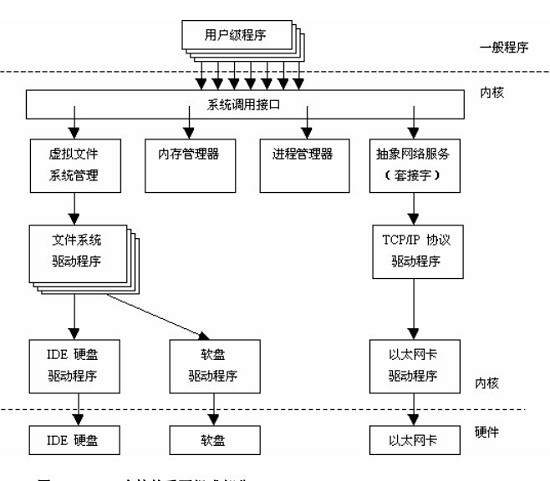
\includegraphics[width=0.8\textwidth]{1.1-1.jpg}
\end{figure}

其中系统调用接口:SCI 层提供了某些机制执行从用户空间到内核的函数调用。

\subsection{Linux 远程登录}

Linux 系统中是通过 ssh 服务实现的远程登录功能,默认 ssh 服务端口号为 22。

安装ssh:yum install ssh

启动ssh:service sshd start

登录远程服务器:ssh -p 50022 my@127.0.0.1

输入密码:my@127.0.0.1:
(-p 后面是端口,my 是服务器用户名,127.0.0.1 是服务器 ip)

回车输入密码即可登录。

\subsection{Linux 进程}

在 Linux 系统中,能够同时运行多个进程,Linux 通过在短的时间间隔内轮流运行这些进程而实现“多任务”。这一短的时间间隔称为“时间片”,让进程轮流运行的方法称为“进程调度” ,完成调度的程序称为调度程序。

Linux 中常见的进程间通讯机制有信号、管道、共享内存、信号量和套接字等。

\subsubsection{相关命令}

可以使用\$ps命令来查询正在运行的进程,比如\$ps -e、-o pid,-o comm,-o cmd,

其中-e表示列出全部进程,-o pid,-o comm,-o cmd分别表示需要PID,COMMAND,CMD信息。

三个信息的意义依次为:PID(process IDentity)是每一个进程的身份(唯一),是一个整数,进程也可以根据PID来识别其他的进程;COMMAND是这个进程的简称;CMD是进程所对应的程序以及运行时所带的参数。

\subsubsection{Linux进程的产生}

当计算机开机的时候,内核(kernel)只建立了一个init进程。Linux内核并不提供直接建立新进程的系统调用。其他所有进程都是init进程通过fork机制建立的。

fork表示:新的进程要通过老的进程复制自身得到,它是一个系统调用。进程存活于内存中。每个进程都在内存中分配有属于自己的一片空间 (address space)。当进程fork的时候,Linux在内存中开辟出一片新的内存空间给新的进程,并将老的进程空间中的内容复制到新的空间中,此后两个进程同时运行。

老进程成为新进程的父进程(parent process),而相应的,新进程就是老的进程的子进程(child process)。一个进程除了有一个PID之外,还会有一个PPID(parent PID)来存储的父进程PID。如果我们循着PPID不断向上追溯的话,总会发现其源头是init进程。所以说,所有的进程也构成一个以init为根的树状结构。

\subsubsection{Linux进程的消失}

当子进程终结时,它会通知父进程,并清空自己所占据的内存,并在内核里留下自己的退出信息(exit code,如果顺利运行,为0;如果有错误或异常状况,为>0的整数)。在这个信息里,会解释该进程为什么退出。

父进程在得知子进程终结时,有责任对该子进程使用wait系统调用。这个wait函数能从内核中取出子进程的退出信息,并清空该信息在内核中所占据的空间。

但是,如果父进程早于子进程终结,子进程就会成为一个孤儿(orphand)进程。孤儿进程会被过继给init进程,init进程也就成了该进程的父进程。init进程负责该子进程终结时调用wait函数。

注意:在Linux中,线程只是一种特殊的进程。多个线程之间可以共享内存空间和IO接口。所以,进程是Linux程序的唯一的实现方式。

\subsubsection{轻量化进程LWP}

与普通进程相比,LWP与其他进程共享所有(或大部分)它的逻辑地址空间和系统资源;与线程相比,LWP有它自己的进程标识符,并和其他进程有着父子关系。另外,线程既可由应用程序管理,又可由内核管理,而LWP只能由内核管理并像普通进程一样被调度。

默认情况下,对于一个拥有n个线程的程序,启动多少轻进程,由哪些轻进程来控制哪些线程由操作系统来控制,这种状态被称为非绑定的状态。因此线程结束后并不会主动释放资源。

而指定了某个线程“绑”在某个轻进程上,就称之为绑定的状态。被绑定的线程具有较高的响应速度,绑定线程可以保证在需要的时候它总有一个轻进程可用。

\subsection{Linux 线程}

https://blog.csdn.net/networkhunter/article/details/100218945

需要头文件:

\#include <pthread.h> 

编译方式:

\$ gcc thread.c -o thread -lpthread

CMakeList.txt中需要加入如下内容来添加链接库:

find\_package(Threads)

target\_link\_libraries( … \${CMAKE\_THREAD\_LIBS\_INIT})

\subsubsection{pthread\_create函数}

\paragraph{函数概述:}~{}

\begin{itemize}
    \item 功能:创建线程(实际上就是确定调用该线程函数的入口点)。
    \item 返回值:返回0表示成功,返回-1表示出错。
    \item 范围限制:主线程,子线程属性设置完成之后。
    \item 注意:无。
\end{itemize}

\paragraph{函数声明:}~{}

int pthread\_create(pthread\_t *thread, const pthread\_attr\_t *attr,

void *(*start\_routine)(void*), void *arg); 

\begin{itemize}
    \item thread:\textcolor{red}{线程句柄},指针,指向线程标识符的指针。 
    
    当一个新的线程调用成功之后,就会通过这个参数将线程的句柄返回给调用者,以便对这个线程进行管理。 

    类型为:pthread\_t。注意传入的是地址。

    \item attr:\textcolor{red}{线程属性对象}。指针类型,这个参数是可选的,默认属性下为NULL,表示非分离属性。以下众多函数均与线程属性有关。
    
    也可以自己设置,类型为:const pthread\_attr\_t。注意传入的也是地址。

    属性总览:

    typedef struct\{

    \qquad int \qquad detachstate;   线程的分离状态

    \qquad int \qquad schedpolicy;  线程调度策略

    \qquad structsched\_param \qquad schedparam;  线程的调度参数

    \qquad int \qquad inheritsched;  线程的继承性

    \qquad int \qquad scope;       线程的作用域

    \qquad size\_t \qquad guardsize;   线程栈末尾的警戒缓冲区大小

    \qquad int \qquad stackaddr\_set;

    \qquad void* \qquad stackaddr;   线程栈的位置

    \qquad size\_t \qquad stacksize;    线程栈的大小

    \}pthread\_attr\_t;

    \item start\_routine():入口函数,线程运行函数的地址。传入函数名即可。
    
    当程序调用了这个接口之后,就会产生一个线程,而这个线程的入口函数就是start\_routine()。如果线程创建成功,这个接口会返回0。 

    \item arg:入口函数参数指针,即指多线程要运行函数的参数。注意传入的是地址。
    
    注意:
    
    {
        \begin{itemize}
            \item 入口函数参数只能是一个void *型的指针,即只能通过结构体封装超过一个以上的参数作为一个整体传递。或者使用类中的this指针。(this指针:每一个对象都能通过 this 指针来访问自己的地址。this 指针是所有成员函数的隐含参数。因此,在成员函数内部,它可以用来指向调用对象)
            \item 不论是函数调用还是线程内外使用,\textcolor{red}{必须对参数进行强制类型转换(void *)}。
            \item 入口函数的返回值也同样必须是一个void *类型的指针,即为传入的参数。这个返回值可以通过pthread\_join()接口获得。
        \end{itemize}
    }
    
\end{itemize}

使用示例: ret = pthread\_create( \&th, NULL, thread, \&arg );  

\subsubsection{pthread\_attr\_init函数---属性的初始化}

\paragraph{函数概述:}~{}

\begin{itemize}
    \item 功能:初始化一个线程属性对象。
    \item 返回值:0成功,非0失败。
    \item 范围限制:主线程函数,创建线程之前。
    \item 注意:在对线程进行处理之前必须进行初始化。调用该函数之后,线程属性结构所包含的内容就是操作系统实现支持的线程所有属性的\textbf{默认值}。
\end{itemize}

\paragraph{函数声明:}~{}

int pthread\_attr\_init(pthread\_attr\_t *attr);

\begin{itemize}
    \item attr:是一个线程属性对象。地址。定义类型为pthread\_attr\_t。
\end{itemize}

使用示例:pthread\_attr\_init(\&attr);

\subsubsection{pthread\_attr\_destroy函数---属性的销毁}

\paragraph{函数概述:}~{}

\begin{itemize}
    \item 功能:销毁一个线程属性对象。删除初始化期间分配的存储空间。
    \item 返回值:0成功,非0失败。
    \item 范围限制:主线程,join之后。
    \item 注意:无。
\end{itemize}

\paragraph{函数声明:}~{}

int pthread\_attr\_destroy(pthread\_attr\_t *attr);

\begin{itemize}
    \item attr:是一个线程属性对象。地址。
\end{itemize}

使用示例:pthread\_attr\_destroy(\&tattr);


\subsubsection{pthread\_join函数---分离属性:线程合并}

\paragraph{函数概述:}~{}

\begin{itemize}
    \item 功能:子线程合入主线程,主线程阻塞等待子线程结束,然后回收子线程资源。避免内存泄漏。
    \item 返回值:0成功,非0失败。
    {
        \begin{itemize}
            \item ESRCH: 没有找到与给定的线程ID相对应的线程。(如果多个线程等待同一个线程终止,则所有等待线程将一直等到目标线程终止。然后一个等待线程成功返回。其余的等待线程将失败返回ESRCH错误)
            \item EDEADLK:将出现死锁,如一个线程等待其本身,或者线程A和线程B 互相等待。
            \item EINVAL:与给定的线程ID相对应的线程是分离线程。
        \end{itemize}
    }
    \item 范围限制:主线程函数,需等待子线程执行结束位置。
    \item 注意:
    {
        \begin{itemize}
            \item 非分离线程属性下,只有在主线程调用该函数时,该线程才会释放自己的资源。
            \item 多线程编程中往往以for循环的形式调用该函数。
            \item 该函数会让主线程阻塞,直到所有线程都已经退出。
            \item 线程合并和分离必须二选一。
        \end{itemize}
    }
    
\end{itemize}

\paragraph{函数声明:}~{}

int pthread\_join(pthread\_t thread, void **status);

\begin{itemize}
    \item thread:需要等待的线程,指定的线程必须位于当前的进程中,而且不得是分离属性的线程。不需要写为线程的地址。
    \item status:线程thread所执行的函数返回值存放地址(返回值地址需要保证有效),其中status可以为NULL。需要强制类型转换(void **)\&。
    
    注意:在主函数中定义,类型与入口函数的参数类型一致即可。

\end{itemize}

使用示例:pthread\_join(th, (void**)\&thread\_ret );  

\subsubsection{pthread\_detach函数---分离属性:线程分离}

\paragraph{函数概述:}~{}

\begin{itemize}
    \item 功能:设置分离属性,使主线程与子线程分离,子线程结束后,资源自动回收。
    \item 返回值:调用成功完成之后返回零。其他任何返回值都表示出现了错误:
    
    EINVAL:thread是分离线程;

    ESRCH:thread不是当前进程中有效的为分离线程。

    \item 范围限制:子线程中,函数开头位置设置。
    \item 注意:调用该函数后,入口函数结束时自动回收资源,不用调用pthread\_join()。往往适用于不需要主线程等待的情况。
\end{itemize}

\paragraph{函数声明:}~{}

int pthread\_detach(pthread\_t thread);

\begin{itemize}
    \item thread:线程标识符。
\end{itemize}

使用示例:pthread\_detach(pthread\_self());其中\textcolor{red}{pthread\_self()是获得自身线程标识符函数}。

\subsubsection{pthread\_attr\_setdetachstate函数---分离属性}

用来决定一个线程以什么样的方式来终止自己,何时释放自己的资源。

\paragraph{函数概述:}~{}

\begin{itemize}
    \item 功能:分离属性就是让线程在创建之前就决定它应该是分离的。如果设置了这个属性,就没有必要调用pthread\_join()或pthread\_detach()来回收线程资源了。 
    \item 返回值:成功返回0,若失败返回-1。
    \item 范围限制:主线程函数,创建线程之前,定义属性后。
    \item 注意:无。
\end{itemize}

\paragraph{函数声明:}~{}

pthread\_attr\_setdetachstate(pthread\_attr\_t *attr, int detachstate); 

\begin{itemize}
    \item attr:是一个线程属性对象。地址。
    \item detachstate:属性,可取值为:
    
    PTHREAD\_CREATE\_DETACHED(分离的)
    
    PTHREAD\_CREATE\_JOINABLE(可合并的,也是默认属性)

\end{itemize}

使用示例:ret = pthread\_attr\_setdetachstate(\&tattr,

PTHREAD\_CREATE\_DETACHED);

\subsubsection{pthread\_attr\_setscope函数---绑定属性}

绑定属性:指一个用户线程固定地分配给一个内核线程。

\paragraph{函数概述:}~{}

\begin{itemize}
    \item 功能:设置线程的绑定属性。
    \item 返回值:0成功,-1失败。
    \item 范围限制:主线程函数,分离属性之后。
    \item 注意:Linux的线程永远都是绑定的,所以非绑定状态在Linux中不管用,而且会返回ENOTSUP错误。设置为绑定状态后则不能重新设置为非绑定状态。
\end{itemize}

\paragraph{函数声明:}~{}

int pthread\_attr\_setscope(pthread\_attr\_t *attr, int scope);

\begin{itemize}
    \item attr:线程属性对象的指针,传入的是地址,定义类型为pthread\_attr\_t。
    \item scope:传入类型。包括:
    {
        \begin{itemize}
            \item PTHREAD\_CREATE\_DETACHED:绑定状态;
            \item PTHREAD\_CREATE\_JOINABLE:非绑定状态;
        \end{itemize}
    }
\end{itemize}

使用示例:pthread\_attr\_setscope(\&attr, PTHREAD\_SCOPE\_SYSTEM); 

\subsubsection{pthread\_attr\_setschedpolicy函数---调度属性(算法)}

线程的调度属性有三个,分别是:算法、优先级和继承权。

算法:Linux提供的线程调度算法有三个:轮询、先进先出和其它。

\begin{itemize}
    \item 轮询:指时间片轮转,当线程的时间片用完,系统将重新分配时间片,并将它放置在就绪队列尾部,以保证具有相同优先级的轮询任务获得公平的CPU占用时间。
    \item 先进先出:就是先到先服务,一旦线程占用了CPU则一直运行,直到有更高优先级的线程出现或自己放弃。
    \item 其他:代表采用Linux自己认为更合适的调度算法,默认算法。
    \item 注意:其中轮询和先进先出调度算法是POSIX标准所规定,属于实时调度算法。
    
\end{itemize}

\paragraph{函数概述:}~{}

\begin{itemize}
    \item 功能:设置线程调度算法的接口。
    \item 返回值:成功则返回0,失败返回其他值。
    \item 范围限制:主线程函数,绑定属性之后。
    \item 注意:无。
\end{itemize}

\paragraph{函数声明:}~{}

pthread\_attr\_setschedpolicy(pthread\_attr\_t *attr, int policy);

\begin{itemize}
    \item attr:是一个线程属性对象。地址。
    \item policy:线程调度策略属性值中指定的值。可为:
    
    SCHED\_RR(轮询)
    
    SCHED\_FIFO(先进先出)
    
    SCHED\_OTHER(其它)

\end{itemize}

使用示例:pthread\_attr\_setschedpolicy(\&attr[i], SCHED\_FIFO);  

\subsubsection{pthread\_attr\_setschedparam函数---调度属性(优先级)}

优先级是从1到99的数值,数值越大代表优先级越高。

只有采用SHCED\_RR或SCHED\_FIFO调度算法时,优先级才有效。其他情况下,优先级恒为0。

\paragraph{函数概述:}~{}

\begin{itemize}
    \item 功能:设置线程优先级的接口。
    \item 返回值:成功则返回0,失败返回其他值。
    \item 范围限制:主线程函数,创建线程之前,调度算法之后。
    \item 注意:如果要设置这个值,需满足:进程必须是以root账号运行的;需要放弃线程的继承权。
\end{itemize}

\paragraph{函数声明:}~{}

int pthread\_attr\_setschedparam(pthread\_attr\_t *attr, struct sched\_param *param)

\begin{itemize}
    \item attr:是一个线程属性对象。地址。
    \item param:结构体,其sched\_priority字段就是线程的优先级。
    
    使用方式:
    
    struct sched\_param param;  

    param.sched\_priority = 20;  

\end{itemize}

使用示例:pthread\_attr\_setschedparam(\&attr[i], param ); 

\subsubsection{pthread\_attr\_setinheritsched函数---调度属性(继承权)}

\paragraph{函数概述:}~{}

\begin{itemize}
    \item 功能:设置线程继承权的接口。
    \item 返回值:成功则返回0,失败返回其他值。
    \item 范围限制:主线程函数,调度优先级之后。
    \item 注意:无。
\end{itemize}

\paragraph{函数声明:}~{}

int pthread\_attr\_setinheritsched(pthread\_attr\_t *attr, int inheritsched);  

\begin{itemize}
    \item atttr:是一个线程属性对象。地址。
    \item inheritsched:有两个取值:
    
    PTHREAD\_INHERIT\_SCHED(拥有继承权)(默认)
    
    PTHREAD\_EXPLICIT\_SCHED(放弃继承权)

\end{itemize}

使用示例:pthread\_attr\_setinheritsched(\&attr[i], PTHREAD\_EXPLICIT\_SCHED);

\subsubsection{pthread\_attr\_setstacksize函数---作用域属性}

\paragraph{函数概述:}~{}

\begin{itemize}
    \item 功能:修改线程堆栈大小属性的接口。
    \item 返回值:0成功,非0失败。
    \item 范围限制:主线程函数,创建线程之前,调度属性之后。
    \item 注意:Linux系统为每个线程默认分配了8MB的堆栈空间,如果觉得这个空间不够用,可以通过修改线程的堆栈大小属性进行扩容。 
\end{itemize}

\paragraph{函数声明:}~{}

int pthread\_attr\_setstacksize(pthread\_attr\_t *attr, size\_t stacksize); 

\begin{itemize}
    \item attr:是一个线程属性对象。地址。
    \item stacksize:堆栈大小,以字节为单位。需要注意的是,线程堆栈不能小于16KB,而且尽量按4KB(32位系统)或2MB(64位系统)的整数倍分配,也就是内存页面大小的整数倍。
\end{itemize}

使用示例:略。

\subsubsection{pthread\_attr\_setguardsize函数---满栈警戒区属性}

\paragraph{函数概述:}~{}

警戒区:

为了防止线程的堆栈用满,Linux为线程堆栈设置了一个满栈警戒区。这个区域一般就是一个页面,属于线程堆栈的一个扩展区域。一旦有代码访问了这个区域,就会发出SIGSEGV信号进行通知。

\begin{itemize}
    \item 功能:修改满栈警戒区属性的接口。
    \item 返回值:0成功,非0失败。
    \item 范围限制:主线程函数,创建线程之前,作用域之后。
    \item 注意:如果修改了线程堆栈的大小,那么系统会认为用户会自己管理堆栈,也会将警戒区取消掉,如果有需要就要开启它。 
\end{itemize}

\paragraph{函数声明:}~{}

int pthread\_attr\_setguardsize(pthread\_attr\_t *attr, size\_t guardsize); 

\begin{itemize}
    \item attr:是一个线程属性对象。地址。
    \item guardsize:警戒区大小了,以字节为单位。与设置线程堆栈大小属性相仿,应该尽量按照4KB或2MB的整数倍来分配。当设置警戒区大小为0时,就关闭了这个警戒区。 
\end{itemize}

使用示例:略。

获取栈溢出保护区大小:

int pthread\_attr\_getguardsize(pthread\_attr\_t *attr, size\_t guardsize)

其中第二个参数为输出的单位,1表示1字节。

\subsubsection{线程本地存储}

Thread Local Storage,简称TLS,线程私有的全局变量,用于避免全局变量的值(如error)被所有子线程修改,导致不确定性的问题。

\paragraph{私有化全局变量方法}~{}

在全局变量的定义前增加 \_\_thread 即可。这样每个线程都有一个自己私有的全局变量g,子线程对值的修改不影响主线程的值,主线程也不影响子线程的值。


\paragraph{pthread\_key\_create函数}~{}

int pthread\_key\_create(pthread\_key\_t *key, void (*destructor)(void*));

\begin{itemize}
    \item 功能:用于创建一个线程本地存储区。
    \item 返回值:0成功,非0失败。
    \item 范围限制:主线程函数,创建线程之前。
    \item 注意:参数涉及强制类型转换。内部函数需要通过指针赋值方式来释放私有化全局变量。
    \item 参数:
    {
        \begin{itemize}
            \item key : 用来返回这个存储区的句柄,需要使用一个全局变量保存,以便所有线程都能访问到。类型:pthread\_key\_t。传入地址。 
            \item  *destructor : 指明了一个destructor函数,如果这个参数不为空,那么当每个线程结束时,系统将调用这个函数来释放绑定在这个键上的内存块,否则可以传递NULL。类型必须为void *,参数也需为void *。
        \end{itemize}
    }
\end{itemize}

\paragraph{pthread\_key\_delete函数}~{}

int pthread\_key\_delete(pthread\_key\_t key);

\begin{itemize}
    \item 功能:用于回收线程本地存储区。
    \item 返回值:0成功,非0失败。
    \item 范围限制:主线程函数,线程回收之后。
    \item 注意:无。
    \item 参数:唯一的参数就要回收的存储区的句柄。
\end{itemize}

\paragraph{pthread\_getspecific函数}~{}

void* pthread\_getspecific(pthread\_key\_t key);  

\begin{itemize}
    \item 功能:用于获取线程本地存储区的数据。
    \item 返回值:0成功,非0失败。
    \item 范围限制:子线程中。
    \item 注意:无。
    \item 参数:句柄。
\end{itemize}

\paragraph{pthread\_setspecific函数}~{}

int pthread\_setspecific(pthread\_key\_t key, const void *value);

\begin{itemize}
    \item 功能:用于设置线程本地存储区的数据。
    \item 返回值:0成功,非0失败。
    \item 范围限制:子线程中,使用该值前。
    \item 注意:无。
    \item 参数:
    {
        \begin{itemize}
            \item key:句柄。
            \item value:需要采用本地存储区的值的指针,不需要强制类型转换,不需要常量,类型thread\_data\_t *。
        \end{itemize}
    }
\end{itemize}

\subsection{线程的同步}

Linux提供的线程同步机制主要有互斥锁和条件变量。

\subsubsection{互斥锁}

用来保证多线程的共享数据的完整性,即在一个线程操作某共享数据时对其上锁,使其他的线程无法对该数据进行操作。

\paragraph{特点:}~{}
\begin{itemize}
    \item 原子性:把一个互斥量锁定为一个原子操作,如果一个线程锁定了一个互斥量,没有其他线程在同一时间可以成功锁定这个互斥量;
    \item 唯一性:如果一个线程锁定了一个互斥量,在它解除锁定之前,没有其他线程可以锁定这个互斥量;
    \item 非繁忙等待:如果一个线程已经锁定了一个互斥量,第二个线程又试图去锁定这个互斥量,则第二个线程将被挂起(不占用任何cpu资源),直到第一个线程解除对这个互斥量的锁定为止,第二个线程则被唤醒并继续执行,同时锁定这个互斥量。
    \item 使用互斥锁会影响代码的执行效率,多任务改成了单任务执行。这段代码称为临界区。
\end{itemize}

\paragraph{死锁}~{}

两个线程已经各自拥有一把锁了,但是还想得到对方的锁,这个时候两个线程都会被暂停,称为死锁。

\paragraph{互斥锁基本函数}~{}

\begin{itemize}
    \item pthread\_mutex\_init(A,B) //初始化互斥锁[主函数]
    
    A:pthread\_mutex\_t *restrict mutex:指向互斥量的指针,类型为pthread\_mutex\_t,传入地址。

    pthread\_mutex\_t mutex = PTHREAD\_MUTEX\_INITIALIZER;//定义

    B:const pthread\_mutexattr\_t *restrict attr:指向互斥量属性的指针,NULL即可。

    \item pthread\_mutex\_destroy(A) //销毁互斥锁[主函数]
    \item pthread\_mutex\_lock(A) //互斥锁获得锁[子线程]
    \item pthread\_mutex\_trylock(A) //尝试获得锁[子线程]

    如果该互斥锁已经锁定,则返回一个不为的错误值,如果该互斥锁没有锁定,则返回0,表示尝试加锁成功。

    用它试图加锁的线程永远都不会被系统暂停,只是通过返回EBUSY来告诉程序员这个锁已经有人用了。至于是否继续“强闯”临界区,则由程序员决定。

    \item pthread\_mutex\_unlock(A) //释放互斥锁[子线程]
\end{itemize}

\paragraph{注意事项}~{}

\begin{itemize}
    \item 对共享资源操作前一定要获得锁。
    \item 完成操作以后一定要由上锁的进(线)程释放锁释放锁。
    \item 锁并不是与某个具体的变量进行关联,它本身是一个独立的对象。
    \item 在获得锁和释放锁之间的操作可视为单线程的,因此应尽量短时间地占用锁。
    \item 如果有多锁, 如获得顺序是ABC连环扣, 释放顺序也应该是ABC。
    \item 线程错误返回时应该释放它所获得的锁。
\end{itemize}

\subsubsection{条件变量}

条件变量是一种事件机制。由一类线程来\textbf{控制“事件”}的发生,另外一类线程\textbf{等待“事件”}的发生。主要包括两个动作:

一个线程等待"条件变量的条件成立"而挂起暂停;

另一个线程使"条件成立"(给出条件成立信号)。

条件变量必须是\textbf{共享于线程之间的全局变量}。为了防止竞争,条件变量的使用总是和一个互斥锁结合在一起。  

\paragraph{条件变量基本函数}~{}

\begin{itemize}
    \item pthread\_cond\_init(C,D) //初始化条件变量的接口[主函数]
    
    C:pthread\_cond\_t *cond:是一个指向条件变量的指针,类型为pthread\_cond\_t,传入地址。

    pthread\_cond\_t has\_producer = PTHREAD\_COND\_INITIALIZER;//定义

    D:const pthread\_condattr\_t *attr:是一个指向条件变量属性的指针,NULL即可。

    \item pthread\_cond\_destory(C) //销毁条件变量的接口,非释放内存空间[主函数]
    \item pthread\_cond\_signal(C) //控制“事件”发生的接口,激活等待列表中的线程,即广播形式[子线程]
    \item pthread\_cond\_broadcast(C) //控制“事件”发生的接口,激活所有等待线程列表中最先入队的线程,即单播形式[子线程]
    \item pthead\_cond\_wait(C,A) //等待“事件”发生的接口,即等待条件变量,挂起线程,没有信号就一直等待[子线程]
    \item pthread\_cond\_timedwait(C,A,E) //等待“事件”发生的接口,不同之处在于会有timeout时间,如果到了timeout,线程自动解除阻塞[子线程]
    
    E:const timespec *abstime:等待时间(其值为系统时间+等待时间)

\end{itemize}

\paragraph{注意事项}~{}

\begin{itemize}
    \item 函数pthead\_cond\_wait的工作流程为:对于一个已经成功锁定了的进程,首先将本线程休眠,放在等待队列(称为阻塞);然后对本线程的互斥量解锁,接着等待别的线程的解锁信号后去竞争锁(称为唤醒),继续执行线程。(解锁并阻塞是一个原子操作)
    \item 解锁信号:另一个占据了该互斥量的线程在完成了对全局变量的操作后,执行解锁,然后调用thread\_cond\_broadcast或pthread\_cond\_signal函数(广播)。
    \item 但由于解锁信号对应的情况下并不一定与唤起该线程的情况相同,则往往在调用pthead\_cond\_wait时会加入一个额外的判断来确定是否还需要等待。
    \item 判断可以采用if的形式,也可以采用while的形式。前者在总计只有2个线程的情况下与后者相同。否则前者在下次竞争不到锁的时候就会继续执行线程的操作,而后者则会一直等待下去。
    \item 先发解锁信号再解锁。避免有线程在收到信号前恰好获得锁。
\end{itemize}

\paragraph{与互斥锁关系}~{}

\begin{itemize}
    \item 与互斥锁同时采用,可用于让线程按一定的顺序来操作全局变量数据。即一个线程用互斥锁锁住了某一个操作过程,但如果全局变量不满足条件变量的要求,则会解锁该操作规程,让其他线程来操作。当满足要求时,再锁住操作过程执行。(在此期间一直处于临界区)
    \item pthread\_cond\_wait与thread\_mutex\_lock连用,在线程通过后者获得锁后,如果不满足条件,则调用前者释放锁,并将本线程放在线程等待队列之后。
    \item 额外的解锁条件需要自己编写。
\end{itemize}

\subsubsection{基本流程}

提前需定义的参数:

\begin{itemize}
    \item pthread\_t  //线程对象
    \item pthread\_attr\_t  //线程属性对象
    \item pthread\_key\_t  //本地存储区键
    \item pthread\_mutex\_t mutex = PTHREAD\_MUTEX\_INITIALIZER;  //互斥锁对象
    \item pthread\_cond\_t  cond  = PTHREAD\_COND\_INITIALIZER;  //条件变量对象
\end{itemize}

主线程:

\begin{itemize}
    \item pthread\_attr\_init  //初始化线程属性
    \item pthread\_attr\_setdetachstate //设置分离属性,无join、detach
    \item pthread\_attr\_setscope //设置绑定属性
    \item pthread\_attr\_setschedpolicy //设置调度属性 (算法)
    \item pthread\_attr\_setschedparam //设置调度属性 (优先级)
    \item pthread\_attr\_setinheritsched //设置调度属性 (继承权)
    \item pthread\_attr\_setstacksize //设置作用域属性
    \item pthread\_attr\_setguardsize //设置满栈警戒区属性
    \item pthread\_key\_create //创建线程本地存储区
    \item pthread\_key\_delete //回收线程本地存储区
    \item pthread\_mutex\_init //初始化互斥锁
    \item pthread\_cond\_init //初始化条件变量
    \item pthread\_create //创建线程
    \item pthread\_join  //调用回收线程
    \item pthread\_mutex\_destroy //销毁互斥锁
    \item pthread\_cond\_destory //销毁条件变量
    \item pthread\_attr\_destroy  //销毁线程
\end{itemize}

子线程:

\begin{itemize}
    \item pthread\_detach //自动回收,无join
    \item pthread\_setspecific //设置线程本地存储区的数据
    \item pthread\_getspecific //获取线程本地存储区的数据
    \item pthread\_mutex\_lock //互斥锁获得锁
    \item pthead\_cond\_wait //等待条件变量,挂起线程
    \item 公共操作
    \item pthread\_cond\_signal 或 pthread\_cond\_broadcast 释放解锁信号广播/单播
    \item pthread\_mutex\_unlock //释放互斥锁
\end{itemize}

\subsection{Linux内存管理}

了让有限的物理内存满足应用程序对内存的大需求量,Linux 采用了称为“虚拟内存”的内存管理方式。Linux 将内存划分为容易处理的“内存页”(对于大部分体系结构来说都是 4KB)。Linux 包括了管理可用内存的方式,以及物理和虚拟映射所使用的硬件机制。

\subsection{Linux文件系统}

Linux系统能支持多种目前流行的文件系统,如EXT2、 EXT3、 FAT、 FAT32、 VFAT和ISO9660。

Linux下面的文件类型主要有:

1) 普通文件:C语言元代码、SHELL脚本、二进制的可执行文件等。分为纯文本和二进制;

2) 目录文件:目录,存储文件的唯一地方;

3) 链接文件:指向同一个文件或目录的的文件;

4) 设备文件:与系统外设相关的,通常在/dev下面。分为块设备和字符设备;

5)管道(FIFO)文件: 提供进程之间通信的一种方式;

6)套接字(socket) 文件: 该文件类型与网络通信有关;

可参考:https://www.linuxprobe.com/linux-system-structure.html

\subsection{Linux防火墙}

\subsubsection{常用命令}

\begin{itemize}
    \item 启动:systemctl start firewalld
    \item 重启:systemctl restart firewalld
    \item 停止:systemctl stop firewalld
    \item 重新加载:firewall-cmd --reload
    \item 查看firewalld的运行状态:
    
        firewall-cmd --state

    \item 取消开放https服务,即禁止https服务:
    
        firewall-cmd --zone=drop --remove-service=https

    \item 开放22端口:
    
        firewall-cmd --zone=drop --add-port=22/tcp

    \item 取消开放22端口:
    
        firewall-cmd --zone=drop --remove-port=22/tcp

    \item 开放两个端口:
    
    firewall-cmd --zone=drop --add-port=8080-8081/tcp

    \item 查询drop区域开放了哪些端口:
    
    firewall-cmd --zone=drop --list-ports

    \item 其他常用命令:
    
    允许icmp协议流量,即允许ping:

    firewall-cmd --zone=drop --add-protocol=icmp

    取消允许icmp协议的流量,即禁ping:

    firewall-cmd --zone=drop --remove-protocol=icmp
    
    查询drop区域开放了哪些协议:

    firewall-cmd --zone=drop --list-protocols

    将原本访问本机888端口的流量转发到本机22端口:
    
    firewall-cmd --zone=drop --add-forward-port
    =port=888:proto=tcp:toport=22
\end{itemize}


\section{socket基础}

\subsection{socket通信的概念}

套接字,运行在计算机中的两个程序通过socket建立起一个通道,数据在通道中传输。套接字可以看成是两个网络应用程序进行通信时,各自通信连接中的端点,这是一个逻辑上的概念。它是网络环境中进程间通信的API(应用程序编程接口)(是IP地址和端口结合)。

socket把复杂的TCP/IP协议族隐藏了起来,只要用好socket相关的函数,就可以完成网络通信。

\subsection{socket的分类}

socket提供了流(stream)和数据报(datagram)两种通信机制,即流socket和数据报socket。

流socket基于TCP协议,是一个有序、可靠、双向字节流的通道,传输数据不会丢失、不会重复、顺序也不会错乱。类似于打电话。

数据报socket基于UDP协议,不需要建立和维持连接,可能会丢失或错乱。UDP不是一个可靠的协议,对数据的长度有限制,但是它的速度比较高。类似于短信。

在实际开发中,数据报socket的应用场景极少。

\subsection{socket通信的过程}

\subsubsection{服务端}

\begin{itemize}
    \item 创建服务端的socket。socket()
    \item 把服务端指定的用于通信的ip地址和端口绑定到socket上。bind()
    \item 把socket设置为监听模式,以监听用户请求。listen()
    \item 接受客户端的连接。accept()
    \item 与客户端通信,接收客户端发过来的报文后,回复处理结果。send()/recv()
    \item 不断的重复上一步步,直到客户端断开连接。
    \item 关闭socket,释放资源。close()
\end{itemize}

\subsubsection{客户端}

\begin{itemize}
    \item 创建客户端的socket。socket()
    \item 向服务器发起连接请求。connect()
    \item 与服务端通信,发送一个报文后等待回复,然后再发下一个报文。send()/recv()
    \item 不断的重复上一步,直到全部的数据被发送完。
    \item 关闭socket,释放资源。close()
\end{itemize}

\begin{figure}[htb!]%插入图片
    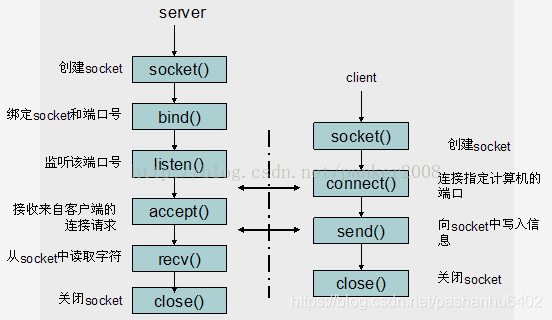
\includegraphics[width=0.8\textwidth]{2.3-1.png}
\end{figure}

\subsection{Socket}

在Linux系统中,一切输入输出设备皆文件。而socket本质上可以视为一种特殊的文件,即通信的实现,因此socket的通信过程也可以理解为通过“打开open –> 读写write/read –> 关闭close”模式的操作过程。

注意:

a. 客户端有一个socket,是用于发送报文的socket;而服务端有两个socket,一个是用于监听的socket,还有一个就是客户端连接成功后,由accept函数创建的用于与客户端收发报文的socket。

b. socket是系统资源,操作系统打开的socket数量是有限的,在程序退出之前必须关闭已打开的socket,就像关闭文件指针一样,就像delete已分配的内存一样,极其重要。

c. 关闭socket的代码不能只在main函数的最后,那是程序运行的理想状态,还应该在main函数的每个return之前关闭。

d. socket类型的servaddr的地址的强制转换,(struct sockaddr *)\&servaddr。

\subsection{Socket主要参数及结构体}

\subsubsection{socket函数返回的值}

返回值称为socket描述符(socket descriptor),其本质是一个文件描述符,是一个整数。把它作为参数,通过它来进行一些读写操作。

0表示标准输入,1表示标准输出,2表示标准错误。

注意:默认创建的socket是主动连接的。

\subsubsection{有关定义}

\begin{itemize}
    \item 大端模式、小端模式:“大端”和”小端”表示多字节值的哪一端存储在该值的起始地址处;小端存储在起始地址处,即是小端字节序;大端存储在起始地址处,即是大端字节序。
    
    a. 大端字节序(Big Endian):最高有效位存于最低内存地址处,最低有效位存于最高内存处;
   
    b. 小端字节序(Little Endian):最高有效位存于最高内存地址,最低有效位存于最低内存处。

    \item 网络字节序NBO:网络字节序是大端字节序。在进行网络传输的时候,发送端发送的第一个字节是高位字节。
    \item 主机字节序HBO:不同的机器HBO不相同,与CPU的设计有关,数据的顺序是由CPU决定的,而与操作系统无关。不同体系结构的机器之间不能直接通信,所以要转换成一种约定的顺序,也就是网络字节顺序。存在专门的函数来进行二者的转换。
    \item 转换函数命名规则:h主机、n是网络字节序,to是转换为,s是短型数据,l是长型。
    \item 命名规则:
    
    socket字符:sockfd客户端,listenfd服务端;

    网络地址:clientaddr客户端,servaddr服务端;
    \item 待添加

\end{itemize}

\subsubsection{struct hostent* h}

域名和网络地址结构体:

struct hostent

\{

\qquad    char *h\_name;  //主机名,即官方域名
    
\qquad    char **h\_aliases;  //主机所有别名构成的字符串数组,同一IP可绑定多个域名

\qquad    int h\_addrtype; //主机IP地址的类型,AF\_INET(ipv4)、AF\_INET6(ipv6)

\qquad    int h\_length;  //主机IP地址长度,IPV4为4,IPV6为16。

\qquad    char **h\_addr\_list;  //主机的ip地址,虽然为char形式,但以网络字节序格式存储,可以通过memcpy互相拷贝。

\};

注意:
a. 通常用于客户端已知对方ip情况下获得对方网络其他信息。

b. 与下面的结构体一样,定义时指的是哪个端,其内数据就指哪个端。

c. 具有预定义参数:\# define h\_addr  h\_addr\_list[0]

d. \textcolor{red}{主要用于客户端存入端口和ip地址信息,然后通过h\_addr来将信息传递给网络地址结构体sin\_addr}。

\paragraph{操作函数}~{}


\begin{itemize}
    \item *gethostbyname(const char *name);
    
    用于客户端指定服务端的ip地址,详见后文函数介绍,注意参数为char类型的常量。成功执行该函数后结构体内各变量均可获得。

    \item 新型网路地址转化函数inet\_pton和inet\_ntop:
    
    这两个函数是随IPv6出现的函数,对于IPv4地址和IPv6地址都适用,函数中p和n分别代表表达(presentation)和数值(numeric)。地址的表达格式通常是ASCII字符串,数值格式则是存放到套接字地址结构的二进制值。

    int inet\_pton(int family, const char *strptr, void *addrptr);     //将点分十进制的ip地址转化为用于网络传输的数值格式
        
    返回值:若成功则为1,若输入不是有效的表达式则为0,若出错则为-1。
 
    const char * inet\_ntop(int family, const void *addrptr, char *strptr, size\_t len);     //将数值格式转化为点分十进制的ip地址格式

    返回值:若成功则为指向结构的指针,若出错则为NULL。

    其中:family即主机IP地址的类型参数。
    
\end{itemize}

\subsubsection{struct sockaddr\_in servaddr}

表示地址信息的数据结构(体),存放了目标地址和端口。与结构体sockaddr把目标地址和端口信息混在一起了不同,其把port和addr 分开储存在两个变量中。

struct sockaddr\_in

\{

\qquad sa\_family\_t \quad sin\_family; //协议族,在socket编程中只能是AF\_INET。

\qquad unit16\_t \quad sin\_port; //16位的TCP/UDP端口号。

\qquad struct in\_addr \quad sin\_addr; //32位IP地址

\qquad char \quad sin\_zero[8]; //不使用。

\}

其中:

struct in\_addr 

\{

\qquad in\_addr\_t s\_addr; //32位IP v4地址。

\qquad (可表示为:servaddr.sin\_addr.s\_addr)

\}

\paragraph{操作函数}~{}

\begin{itemize}
    \item inet\_addr():将十进制IP地址字符串转为网络二进制数字(网络字节序),返回的IP地址是网络字节序的。
    
    (const char----> \textcolor{red}{in\_addr\_t})(ascii to network)

    \item inet\_ntoa():将网络二进制数字(网络字节序)转为十进制IP地址字符串。
    
    (\textcolor{red}{in\_addr}---->const char)(network to ascii)

    \item inet\_aton():将十进制IP地址字符串转为网络二进制数字(网络字节序),与inet\_addr的区别是,结果不是作为返回值,而是保存形参inp所指的in\_addr结构体中(前者需要保存到in\_addr\_t变量中)。
    
    函数原型:int inet\_aton(cont char* cp, struct in\_addr\_t *inp)
    
    (const char----> \textcolor{red}{in\_addr})(ascii to network)

    \item htons()、htonl()作用是将端口号由主机字节序转换为网络字节序的整数值。前者针对的是16位的(short)、后者针对的是32位的(long)。
    
    (int to in\_addr\_t)(host to net)
    
    (不一定是in\_addr\_t,满足要求的字符即可,例如unit16\_t)

    \item 与htonl()和htons()作用相反的两个函数是:ntohl()和ntohs()。
    
    (net to host)
    
    \item 应用:
    
    a. 服务端绑定(自身的)IP地址:

    servaddr.sin\_addr.s\_addr = \textcolor{red}{inet\_addr}("192.168.149.129");  // 指定ip地址  
    
    servaddr.sin\_addr.s\_addr = \textcolor{red}{htonl(INADDR\_ANY)};  // 本主机的任意ip地址。在实际开发中,采用任意ip地址的方式比较多。

    b. 服务端绑定通信端口,也可用于客户端指定服务端的通信端口:
    
    servaddr.sin\_port = \textcolor{red}{htons}(5000);  // 通信端口5000

    \item 注意:htons()的参数为int型的无符号短整形数,若用argv[]来传递,需要强制转换类型函数atoi()。同理htonl()。
    \item 注意:其中sin\_addr和sin\_port的字节序都是网络字节序,而sin\_family不是。因为前者是从IP和UDP协议层取出来的数据,是直接和网络相关的。但sin\_family域只是内核用来判断struct sockaddr\_in是存储的什么类型的数据,且永远不会被发送到网络上,所以可以使用主机字节序来存储。
    \item 注意:不论是那个端的程序采用,servaddr指的是哪个端,端口、IP地址就是哪个端。

\end{itemize}

注意:通常服务器在启动的时候都会绑定一个众所周知的地址(如ip地址+端口号),用于提供服务,客户就可以通过它来接连服务器;而客户端就不用指定,有系统自动分配一个端口号和自身的ip地址组合。这就是为什么通常服务器端在listen之前会调用bind(),而客户端就不会调用,而是在connect()时由系统随机生成一个。

\subsection{客户端服务端函数}

以下为几种常用的接口函数:

\subsubsection{socket函数}

\paragraph{函数概述:}~{}

\begin{itemize}
    \item 功能:用于创建一个新的socket。对应于普通文件的打开操作。
    \item 返回值:成功则返回一个socket描述符,失败返回-1,错误原因存于errno 中。
    \item 范围限制:客户端、服务端。
    \item 注意:无。
\end{itemize}

\paragraph{函数声明:}~{}

int socket (int domain, int type, int protocol);

\begin{itemize}
    \item domain:协议域,又称协议族(family)。协议族决定了socket的地址类型,在通信中必须采用对应的地址。
    
        AF\_INET:决定了要用ipv4地址(32位的)与端口号(16位的)的组合;

        AF\_UNIX:决定了要用一个绝对路径名作为地址。

    \item type:指定socket类型。
    
        流式socket(SOCK\_STREAM)是一种面向连接的socket,针对于面向连接的TCP服务应用。数据报式socket(SOCK\_DGRAM)是一种无连接的socket,对应于无连接的UDP服务应用。

    \item protocol:指定协议。
    
        常用协议有IPPROTO\_TCP、IPPROTO\_UDP、IPPROTO\_STCP、IPPROTO\_TIPC等,分别对应TCP传输协议、UDP传输协议、STCP传输协议、TIPC传输协议。

        注意为0则与type相匹配,与type不能随意匹配。

    \item 正常情况,第一个参数只能填AF\_INET,第二个参数只能填SOCK\_STREAM,第三个参数只能填0。
\end{itemize}

使用示例:\textcolor{red}{int sockfd = socket(AF\_INET,SOCK\_STREAM,0))}

\subsubsection{send函数}

\paragraph{函数概述:}~{}

\begin{itemize}
    \item 功能:把数据通过socket发送给对端。
    \item 返回值:函数返回已发送的字符数。出错时返回-1,错误信息errno被标记。
    \item 范围限制:客户端、服务端。
    \item 注意:就算是网络断开,或socket已被对端关闭,send函数不会立即报错,要过几秒才会报错。如果send函数返回的错误(<=0),表示通信链路已不可用。
\end{itemize}

\paragraph{函数声明:}~{}

ssize\_t send(int sockfd, const void *buf, size\_t len, int flags);

\begin{itemize}
    \item sockfd:已建立好连接的\textcolor{red}{客户端}socket。
    \item buf:需发送数据的内存地址。
    \item len:需发送数据的长度。
    \item flags:填0, 其他数值意义不大。
    {
        \begin{itemize}
        \item MSG\_CONFIRM :用来告诉链路层。
        \item MSG\_DONTROUTE:不要使用网关来发送数据,只发送到直接连接的主机上。通常只有诊断或者路由程序会使用,这只针对路由的协议族定义的,数据包的套接字没有。
        \item MSG\_DONTWAIT :启用非阻塞操作,如果操作阻塞,就返回EAGAIN或EWOULDBLOCK。
        \item MSG\_EOR :当支持SOCK\_SEQPACKET时,终止记录。
        \item MSG\_MORE :调用方有更多的数据要发送。这个标志与TCP或者udp套接字一起使用。
        \item MSG\_NOSIGNAL :当另一端中断连接时,请求不向流定向套接字上的错误发送SIGPIPE,EPIPE 错误仍然返回。
        \item MSG\_OOB:在支持此概念的套接字上发送带外数据(例如,SOCK\_STREAM类型);底层协议还必须支持带外数据。
    \end{itemize}

    }
\end{itemize}

使用示例:\textcolor{red}{iret=send(sockfd,buffer,strlen(buffer),0);}

\subsubsection{recv函数}

\paragraph{函数概述:}~{}

\begin{itemize}
    \item 功能:接收对方socket发送过来的数据。
    \item 返回值:函数返回已接收的字符数。出错时返回-1,失败时不会设置errno的值。
    \item 范围限制:客户端、服务端。
    \item 注意:如果socket的对端没有发送数据,recv函数就会等待,如果对端发送了数据,函数返回接收到的字符数。出错时返回-1。如果socket被对端关闭,返回值为0。如果recv函数返回的错误(<=0),表示通信通道已不可用。
\end{itemize}

\paragraph{函数声明:}~{}

ssize\_t recv(int sockfd, void *buf, size\_t len, int flags);

\begin{itemize}
    \item sockfd:为已建立好连接的\textcolor{red}{客户端}socket。
    \item buf:用于接收数据的内存地址。
    \item len:接收数据的长度,不能超过buf的大小,否则内存溢出。
    \item flags:填0, 其他数值意义不大。同上。
\end{itemize}

使用示例:\textcolor{red}{iret=recv(sockfd,buffer,sizeof(buffer),0);}

\subsubsection{gethostbyname()函数}

\paragraph{函数概述:}~{}

\begin{itemize}
    \item 功能:把ip地址或域名转换为hostent 结构体表达的地址。
    \item 返回值:如果成功,返回一个hostent结构指针,失败返回NULL。
    \item 范围限制:客户端。
    \item 注意:只要地址格式没错,一般不会返回错误。失败时不会设置errno的值。
\end{itemize}

\paragraph{函数声明:}~{}

struct hostent *gethostbyname(const char *name);

\begin{itemize}
    \item name:域名或者主机名,例如"192.168.1.3"、"www.freecplus.net"等。
\end{itemize}

使用示例:\textcolor{red}{struct hostent *h = gethostbyname(argv[1])}

\subsubsection{connect函数}

\paragraph{函数概述:}~{}

\begin{itemize}
    \item 功能:客户端通过调用connect函数来建立客户端socket与服务器的连接。
    \item 返回值:成功则返回0,失败返回-1,错误原因存于errno 中。
    \item 范围限制:客户端。
    \item 注意:如果服务端的地址错了,或端口错了,或服务端没有启动,connect一定会失败。
\end{itemize}

\paragraph{函数声明:}~{}

int connect(int sockfd, const struct sockaddr *addr, socklen\_t addrlen);

\begin{itemize}
    \item sockfd:客户端socket。
    \item *addr:服务端的网络地址(注意\textcolor{red}{const struct sockaddr *类型,需要强制转换)}。
    \item addrlen:服务端网络地址的长度(addr结构体的大小)。
\end{itemize}

使用示例:\textcolor{red}{connect(sockfd, (struct sockaddr *)\&servaddr,sizeof(servaddr))}

\subsubsection{bind函数}

\paragraph{函数概述:}~{}

\begin{itemize}
    \item 功能:服务端把自身用于通信的地址和端口绑定到socket上。
    \item 返回值:成功则返回0,失败返回-1,错误原因存于errno 中。
    \item 范围限制:服务端。
    \item 注意:如果绑定的地址错误,或端口已被占用,bind函数一定会报错,否则一般不会返回错误。
\end{itemize}

\paragraph{函数声明:}~{}

int bind(int sockfd, const struct sockaddr *addr, socklen\_t addrlen);

\begin{itemize}
    \item sockfd:服务端socket。
    \item *addr:服务端的网络地址。(\textcolor{red}{const struct sockaddr *类型的指针,需要使用强制类型转换}。指向要绑定给sockfd的协议地址。存放了服务端用于通信的地址和端口)。
    \item addrlen:服务端网络地址的长度。
\end{itemize}

使用示例:\textcolor{red}{bind(listenfd,(struct sockaddr *)\&servaddr,sizeof(servaddr));}

\subsubsection{listen函数}

\paragraph{函数概述:}~{}

\begin{itemize}
    \item 功能:用于把主动连接socket变为被动连接的socket,使得这个socket可以接受其它socket的连接请求,从而成为一个服务端的socket。调用之后,服务端的socket就可以调用accept来接受客户端的连接请求。
    \item 返回值:0-成功, -1-失败,错误原因存于errno 中。
    \item 范围限制:服务端。
    \item 注意:listen函数一般不会返回错误。
\end{itemize}

\paragraph{函数声明:}~{}

int listen(int sockfd, int backlog);

\begin{itemize}
    \item sockfd:服务端已经被bind过的socket。
    \item backlog:这个参数涉及到一些网络的细节,比较麻烦,填5、10都行,一般不超过30。
\end{itemize}

使用示例:\textcolor{red}{listen(listenfd,5);}

\subsubsection{accept函数}

\paragraph{函数概述:}~{}

\begin{itemize}
    \item 功能:用于服务端接受客户端的连接。
    \item 返回值:成功则返回0,失败返回-1,错误原因存于errno 中。
    \item 范围限制:服务端。
    \item 注意:
    \item 
    a. 函数在等待的过程中,如果被中断或其它的原因,函数返回-1,表示失败,如果失败,可以重新accept。

    b. 函数等待客户端的连接,如果没有客户端连上来,它就一直等待,这种方式称之为阻塞。

    c. 函数等待到客户端的连接后,\textcolor{red}{创建一个新的socket,函数返回值就是这个新的socket,服务端使用这个新的socket和客户端进行报文的收发。}

\end{itemize}

\paragraph{函数声明:}~{}

int accept(int sockfd,struct sockaddr *addr,socklen\_t *addrlen);

\begin{itemize}
    \item sockfd:服务端已经被listen过的socket。
    \item addr:客户端的网络地址(\textcolor{red}{const struct sockaddr *})。如果不需要客户端的地址,可以填0。也可以先定义一个空的客户端地址,然后填进去。
    \item addrlen:客户端网络地址长度,如果addr为0,addrlen也填0。
\end{itemize}

使用示例:\textcolor{red}{clientfd=accept(listenfd,(struct sockaddr *)\&clientaddr,(socklen\_t*)\&socklen);}





\subsubsection{附注:计算大小函数、运算符}

\paragraph{sizeof运算符}~{}

\begin{itemize}
    \item 参数可以是数组、指针、类型、对象、函数等。
    \item 功能是获得保证能容纳实现所建立的最大对象的字节大小。
    \item 不能用来返回动态分配的内存空间的大小。
    \item 返回值为int类型,大小与空间大小有关,跟对象、结构、数组所存储的内容没有关系。
    \item \textcolor{red}{内容区分为指针时,指的是存储该指针所用的空间大小(存储该指针的地址的长度,是长整型,应该为4),而对于数组名字,则返回数组大小。}
\end{itemize}

\paragraph{strlen函数}~{}

\begin{itemize}
    \item 参数必须是字符型指针(char*)(数组名视为指针)。
    \item 功能是返回字符串的长度。
    \item 可以返回动态内存空间大小。
    \item 返回值为int类型,大小与存储的数据内容有关,与空间的大小和类型无关。
    \item 不区分内容是数组还是指针,就读到\\0为止返回长度。且不把\\0计入字符串的长度。
\end{itemize}

\subsubsection{附注:开辟空间函数、运算符}

\paragraph{memset函数}~{}

\begin{itemize}
    \item 声明:void *memset(void *str, int c, size\_t n)
    {
    \begin{itemize}
        \item str:指向要填充的内存块。
        \item c :为每个字节所赋的值。该值以 int 形式传递,但是函数在填充内存块时是使用该值的无符号字符形式。默认0。
        \item n :内存块大小,单位是字节。
    \end{itemize}
    }
    \item 特点:
    {
    \begin{itemize}
        \item 它是以字节为单位进行赋值的。
        \item 用memset对非字符型数组赋初值是不可取的,因为初值并不是数字,而是对应的ASCII码,会造成初始数值改变。(0不受影响)
        \item 可以说是初始化内存的“万能函数”,在统一赋值时比较适合。一般跟sizeof一起使用。
        \item 通常是给数组或结构体进行初始化。一般的变量如 char、int、float、double 等类型的变量直接初始化即可,没有必要用 memset。
    \end{itemize}
    }
    \item 使用示例:memset(str, 0, sizeof(str));
\end{itemize}

\paragraph{malloc函数}~{}

\begin{itemize}
    \item 声明:extern void *malloc(unsigned int num\_bytes);
    {
    \begin{itemize}
        \item num\_bytes:内存块大小。
    \end{itemize}
    }
    \item 特点:
    {
    \begin{itemize}
        \item 需要自己计算字节数。
        \item 返回指向被分配内存空间的指针,本身无类型,需要强转成指定类型的指针。
        \item 只管分配内存,不进行初始化,所以新内存中值是随机的。
        \item 当内存不再使用的时候,应使用free()函数将内存块释放掉。申请后不释放就是内存泄露。一般跟sizeof一起使用。
    \end{itemize}
    }
    \item 使用示例:p=(int*)malloc(sizeof(int)*128);
\end{itemize}

\paragraph{new运算符}~{}

\begin{itemize}
    \item 声明:无
    \item 特点:
    {
    \begin{itemize}
        \item new返回指定类型的指针。
        \item new可以自动计算所需要的大小。
        \item 会进行初始化。
        \item 开辟新空间用。
    \end{itemize}
    }
    \item 使用示例:p=new int;
\end{itemize}



\subsubsection{附注:字符串复制函数}

\paragraph{memcpy函数}~{}

\begin{itemize}
    \item 声明:void *memcpy(void *str1, const void *str2, size\_t n)
    {
    \begin{itemize}
        \item str1:指向用于存储复制内容的目标数组,类型强制转换为 void* 指针。
        \item str2:指向要复制的数据源,类型强制转换为 void* 指针。
        \item n:要被复制的字节数。
    \end{itemize}
    }
    \item 特点:
    {
    \begin{itemize}
        \item 可以用来拷贝任何数据类型的对象。
        \item 可以指定拷贝的数据长度(n来指定)。
        \item 会完整的复制n个字节,不会因为遇到字符串结束'\\0'而结束。
    \end{itemize}
    }
    \item 使用示例:memcpy(b,a,sizeof(b)) -- (b<a)
\end{itemize}

\paragraph{strcpy函数}~{}

\begin{itemize}
    \item 声明:char* strcpy(char* dest, char* src)
    {
    \begin{itemize}
        \item dest:待被复制的数组指针
        \item str2:要复制的字符串。
    \end{itemize}
    }
    \item 特点:
    {
    \begin{itemize}
        \item 只用于字符串复制,并且它不仅复制字符串内容之外,还会复制字符串的结束符。
        \item 复制过程遇到字符串结束'\\0'结束。
    \end{itemize}
    }
    \item 使用示例:p=new int;
\end{itemize}

\subsubsection{附注:sprintf()函数}

int sprintf(char *str, const char *format, ...);

用途:把结果输出到指定的字符串中。

str -- 这是指向一个字符数组的指针,该数组存储了要写入的字符串。

format -- 这是字符串,包含了要被写入到字符串 str 的文本。与之后参数一起使用,类似于格式化输出中\%d、\%f之类的用法。



\subsection{注意事项}

\begin{itemize}
    \item 每一个端,具有一个socket指示符、一个地址信息。
    \item 凡是函数参数含有地址信息的,均需要强制格式化:
    
    (struct sockaddr *)\& + 地址名

    \item 凡是需要网络地址参数的函数,都必须将类型强制转化为\textcolor{red}{(struct sockaddr *)}类型,因为函数在设计时没有考虑sockaddr\_in类型。
    \item 最好recv函数采用sizeof(最大值),send采用strlen(减少不必要的发送量)。
    \item socket缓冲区:每一个socket在被创建之后,系统都会给它分配两个缓冲区,即输入缓冲区和输出缓冲区。一般来说,默认的输入输出缓冲区大小为8K。
    \item send函数并不是直接将数据传输到网络中,而是负责将数据写入输出缓冲区,数据从输出缓冲区发送到目标主机是由TCP协议完成的。数据写入到输出缓冲区之后,send函数就可以返回了。(数据是否发送出去,是否发送成功,何时到达目标主机,都不由它负责了,而是由协议负责。)
    
    recv函数同理,它是从输入缓冲区中读取数据。

    \item 套接字关闭的时候,输出缓冲区的数据不会丢失,会由协议发送到另一方;而输入缓冲区的数据则会丢失。
    \item 数据的发送和接收是独立的,并不是发送方执行一次send,接收方就执行以此recv。recv函数不管发送几次,都会从输入缓冲区尽可能多的获取数据。如果发送方发送了多次信息,接收方没来得及进行recv,则数据堆积在输入缓冲区中,取数据的时候会都取出来。换句话说,recv并不能判断数据包的结束位置。
    \item 在数据进行发送的时候,需要先检查输出缓冲区的可用空间大小,如果可用空间大小小于要发送的数据长度,则send会被阻塞,直到缓冲区中的数据被发送到目标主机,有了足够的空间之后,send函数才会将数据写入输出缓冲区。
    \item TCP协议正在将数据发送到网络上的时候,输出缓冲区会被锁定(生产者消费者问题),不允许写入,send函数会被阻塞,直到数据发送完,输出缓冲区解锁,此时send才能将数据写入到输出缓冲区。
    \item 函数先检查输入缓冲区,如果输入缓冲区中有数据,读取出缓冲区中的数据,否则的话,recv函数会被阻塞,等待网络上传来数据。如果读取的数据长度小于输出缓冲区中的数据长度,没法一次性将所有数据读出来,需要多次执行recv函数,才能将数据读取完毕。
\end{itemize}

\section{}




\paragraph{函数概述:}~{}

\begin{itemize}
    \item 功能:
    \item 返回值:
    \item 范围限制:
    \item 注意:
\end{itemize}

\paragraph{函数声明:}~{}



\begin{itemize}
    \item 
\end{itemize}

使用示例:








\begin{itemize}
    \item 
    \item 
    \item 
\end{itemize}

\end{document}%文章结束
